 \achapter{16}{Coordinate Vectors and Change of Basis} \label{sec:coordinate_vectors}

\vspace*{-17 pt}
\framebox{
\parbox{\dimexpr\linewidth-3\fboxsep-3\fboxrule}
{\begin{fqs}
\item How do we find the coordinate vector of a vector $\vx$ with respect to a basis $\CB = \{\vv_1, \vv_2, \ldots, \vv_n\}$? 
\item What is a change of basis matrix? 
\item Why is a change of basis useful? 
\end{fqs}}}% \hspace*{3 pt}}

\vspace*{13 pt}

\csection{Application: Describing Orbits of Planets}

Consider a planet orbiting the sun (or an object like a satellite orbiting the Earth). According to Kepler's Laws, we assume an elliptical orbit. There are many different ways to describe this orbit, and which description we use depends on our perspective and the application. One important perspective is to make the description of the orbit as simple as possible for earth-based observations. Two problems arise. One is that the earth's orbit and the orbit of the planet do not lie in the same plane. A second problem is that it is complicated to describe the orbit of a planet using the perspective of the plane of the earth's orbit. A reasonable approach, then, is to establish two different coordinate systems, one for the earth's orbit and one for the planet's orbit. We can then use a change of basis to move back and forth from these two perspectives. 


\csection{Introduction}

In this section we will investigate how a basis in $\R^n$ provides a coordinate system in which each vector in $\R^n$ has a unique set of coordinates. In this way, each basis will provide us with a new perspective to visualize $\R^n$. Then we will see how coordinate vectors can allow us to find change of basis matrices that we can use to easily switch between coordinate systems. We begin our analysis of coordinate systems by looking at how a basis in $\R^2$ gives us a different view of $\R^2$. 

\begin{pa} \label{pa:3_e} Two vectors $\vv_1$ and $\vv_2$ are shown in Figure \ref{F:PA_5d_1}. 
\begin{figure}[h]
\begin{center}
\resizebox{!}{2.5in}{\includegraphics{5_d_PA_Coords}}
\end{center}
\caption{Vectors $\vv_1$ and $\vv_2$.}
\label{F:PA_5d_1}
\end{figure}

\be
\item Explain why $\CB = \{\vv_1, \vv_2\}$ is a basis for $\R^2$. 


\item Draw the vector $\vb = -3\vv_1 + 2\vv_2$ in Figure \ref{F:PA_5d_1}. Explain your process. 

\item In part (2) we were given the weights ($-3$ and 2) of the linear combination of $\vv_1$ and $\vv_2$ that produced $\vb$. We call the vector $\left[ \begin{array}{r} -3 \\2 \end{array} \right]$ the \emph{coordinate vector} of $\vb$ with respect to the basis $\{\vv_1, \vv_2\}$.  

Explain why any vector $\vb$ in $\R^2$ can be written as a linear combination of vectors $\vv_1, \vv_2$. This shows that each vector in $\R^2$ has a coordinate vector in the coordinate system defined by $\vv_1$ and $\vv_2$.


\item Since $\{\vv_1, \vv_2\}$ is a basis for $\R^2$, any vector $\vb$ in $\R^2$ has a coordinate vector in the coordinate system defined by $\vv_1$ and $\vv_2$. But we also need to make sure that each vector has a unique coordinate vector. Explain why there is no vector in $\R^2$ which has two different coordinate vectors.

\item We can think of the vectors $\vv_1$ and $\vv_2$ as defining a coordinate system, with $\Span\{\vv_1\}$ as the ``$x$"-axis and $\Span\{\vv_2\}$ as the ``$y$"-axis. Any vector $\vb$ in $\R^2$ can be written uniquely in the form
\[\vb = x_1 \vv_1 + x_2 \vv_2\]
and the weights serve as the coordinates of $\vb$ in the $\vv_1$, $\vv_2$ coordinate system. In this case the coordinate vector $\left[ \begin{array}{c} x_1 \\ x_2 \end{array} \right]$ of $\vb$ with respect to the basis $\CB =\nobreak \{\vv_1, \vv_2\}$ is written as $[\vb]_{\CB}$.

Let $\CB = \left\{ \left[ \begin{array}{r} -1 \\ 4 \end{array} \right], \left[ \begin{array}{c} 2 \\ 0 \end{array} \right]\right\}$. 
	\ba
	\item Show that $\CB$ is a basis for $\R^2$. 

	\item Find $[\vb]_{\CB}$ if $\vb =  \left[ \begin{array}{c} 0 \\ 6 \end{array} \right]$. Draw a picture to illustrate how $\vb$ is expressed as a linear combination of the vectors in $\CB$.


	\ea
	
\ee
\end{pa}



\csection{Bases as Coordinate Systems in $\R^n$}

Bases are useful for many reasons. A basis provides us with a unique representation of the elements in $\R^n$ as linear combinations of the basis vectors in the coordinate system defined by the vectors. 

As we saw in Preview Activity \ref{pa:3_e}, we can think of a basis $\CB$ of $\R^2$ as determining a coordinate system of $\R^2$. For example, let $\CB = \{\vv_1, \vv_2\}$ where $\vv_1 = \left[ \begin{array}{r} 2 \\ -2 \end{array} \right]$ and $\vv_2 = \left[ \begin{array}{c} 1 \\ 3 \end{array} \right]$. The vector $\vb =  \left[ \begin{array}{r} -4 \\ 12 \end{array} \right]$ can be written as $\vb = -3\vv_1 + 2\vv_2$. Figure \ref{F:3_e_1} shows that if we plot the point that is $-3$ units in the $\vv_1$ direction (where a ``unit" is a copy of $\vv_1$) and $2$ units in the $\vv_2$ direction, then the result is the vector from the origin to point defined by $\vb$.
\begin{figure}[h]
\begin{center}
\resizebox{!}{2.5in}{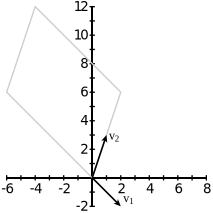
\includegraphics{5_d_Coords_basis}}
\end{center}
\caption{A Coordinate System Defined by a Basis.}
\label{F:3_e_1}
\end{figure}


As discussed in Preview Activity \ref{pa:3_e}, we can think of the vectors $\vv_1$ and $\vv_2$ as defining a coordinate system, with $\Span\{\vv_1\}$ as the ``$x$"-axis and $\Span\{\vv_2\}$ as the ``$y$"-axis. Since $\CB$ is a basis, any vector $\vb$ in $\R^2$ can be written uniquely in the form
\[\vb = x_1 \vv_1 + x_2 \vv_2\]
and the weights serve as the coordinates of $\vb$ in the $\vv_1$, $\vv_2$ coordinate system. We call the vector $\left[ \begin{array}{c} x_1 \\ x_2 \end{array} \right]$ the \emph{coordinate vector} of $\vb$ with respect to the basis $\CB$ and write this vector as $[\vb]_{\CB}$.

This is actually a familiar idea, one we have used for years. The standard coordinates of a vector $\va = \left[ \begin{array}{c} a_1 \\ a_2 \end{array} \right]$ in $\R^2$ are just the coordinates of $\va$ with respect to the standard basis $\{\ve_1, \ve_2\}$ of $\R^2$. 

While we can draw pictures in $\R^2$, there is no reason to restrict this idea to $\R^2$.



\begin{definition} Let $\CB = \{\vv_1, \vv_2, \ldots, \vv_n\}$ be a basis for $\R^n$ for some positive integer $n$. For any vector $\vx$ in $\R^n$, the \textbf{coordinate vector}\index{coordinate vector with respect to a basis in $\R^n$} of $\vx$ with respect to $\CB$ is the vector
\[[\vx]_{\CB} = \left[ \begin{array}{c} x_1 \\ x_2 \\ \vdots \\ x_n \end{array} \right],\]
where
\[\vx = x_1 \vv_1 + x_2 \vv_2 + \cdots + x_n \vv_n.\]
The scalars $x_1$, $x_2$, $\ldots$, $x_n$ are the \textbf{coordinates of the vector}\index{coordinates with respect to a basis in $\R^n$} $\vx$ \textbf{with respect to the basis}.  
\end{definition}

Recall that there is exactly one way to write a vector as a linear combination of basis vectors, so there is only one  coordinate vector of a given vector with respect to a basis. Therefore, the coordinate vector of any vector with respect to a basis is well-defined.

\begin{activity} \label{act:3_e_1} Let $\CS = \{[1 \ 0 \ 0]^{\tr},[0 \ 1 \ 0]^{\tr}, [0 \ 0 \ 1]^{\tr}\}$ and $\CB = \{[1 \ 0 \ 0]^{\tr}, [3 \ 2 \ -1]^{\tr}, [1 \ 1 \ -1]^{\tr}\}$. Assume that $\CS$ and $\CB$ are bases for $\R^3$. Find $\left[\left[ \begin{array}{c} 3\\ 7 \\ 0\end{array} \right]\right]_{\CS}$ and $\left[\left[ \begin{array}{c} 3\\ 7 \\ 0\end{array} \right]\right]_{\CB}$. Note that the coordinate vector depends on the basis that is used. 

\end{activity}

\noindent \textbf{IMPORTANT NOTE:} We have defined the coordinate vector of a vector $\vx$ in $\R^n$ with respect to a basis $\CB = \{\vv_1, \vv_2, \ldots, \vv_n\}$ as the vector $[x_1 \ x_2 \ \ldots \ x_n]^{\tr}$ if 
\[\vx = x_1 \vv_1 + x_2 \vv_2 + \cdots + x_n \vv_n.\]
Until now we have listed a basis as a set without regard to the order in which the basis elements are written. That is, the set $\{\vv_1, \vv_2\}$ is the same as the set $\{\vv_2, \vv_1\}$. Notice, however, that if we change the order of the vectors in our basis, say from $\{\vv_1, \vv_2, \ldots, \vv_n\}$ to  $\{\vv_2, \vv_1, \vv_3, \ldots, \vv_n\}$, then the coordinate vector of $\vx$ with respect to $\CB$ will be different. To avoid this problem, when discussing coordinate vectors we will consider our bases to be \emph{ordered bases}, so that the order in which we write the elements in our basis is fixed. So, for example, the ordered basis $\{\vv_1, \vv_2, \ldots, \vv_n\}$ is different than the ordered basis $\{\vv_2, \vv_1, \vv_3, \ldots, \vv_n\}$. 

Coordinate vectors behave nicely with respect to addition and multiplication by scalars. The next activity illustrates this in $\R^2$. 

\begin{activity} \label{act:3_e_coor_vect_props} Let $\CB = \{\vb_1, \vb_2\}$ be a basis for $\R^2$. Let $\vv$ and $\vw$ be vectors in $\R^2$ with $[\vv]_{\CB} = [x_1 \ x_2]^{\tr}$ and $[\vw]_{\CB} = [y_1 \ y_2]^{\tr}$. 
\ba
\item Determine the components of the vector $[ \vv + \vw]_{\CB}$. How is $[ \vv + \vw]_{\CB}$ related to $[ \vv]_{\CB}$ and $[\vw]_{\CB}$? 

\item Let $c$ be any scalar. Determine the components of the vector $[ c\vv]_{\CB}$. How is $[ c\vv]_{\CB}$ related to $c$ and $[ \vv]_{\CB}$ 

\ea

\end{activity} 

Activity \ref{act:3_e_coor_vect_props} suggests that the following theorem is true for coordinate vectors. The verification is left to the exercises.

\begin{theorem} \label{thm:3_e_coord_vector} Let $n$ be a positive integer and let $\CB$ be a basis for $\R^n$. If $\vv$ and $\vw$ are in $\R^n$ and $a$ and $b$ are any scalars, then 
\[[a\vv+b\vw]_{\CB} = a[\vv]_{\CB} + b[\vw]_{\CB}.\]
\end{theorem} 


\csection{Change of Basis in $\R^n$}

In calculus we change coordinates, from rectangular to polar, for example, to make certain calculations easier. In order for us to be able to work effectively in different coordinate systems, and to easily change back and forth as needed, we will want to have a way to effectively transition from one coordinate system to another. In other words, if we have two different bases for $\R^n$, we want a straightforward way to translate between the coordinate vectors of any given vector in $\R^n$ with respect to the two bases. 


\begin{pa} \label{pa:3_e_2} ~
\be
\item Let $\vb_1 = [4 \ 2]^{\tr}$, $\vb_2 = [-6 \ 8]^{\tr}$, $\vc_1 = [1 \ 1 ]^{\tr}$, $\vc_2 = [1 \ -1]^{\tr}$, and let $\CB = \{\vb_1, \vb_2\}$ and $\CC = \{\vc_1, \vc_2\}$.
	\ba
	\item Show that $\CB$ and $\CC$ are bases for $\R^2$. 
	

	\item Let $\vv = 3 \vb_1 + 2 \vb_2$. What is $[\vv]_{\CB}$?

	\item Since $\CC$ is also a basis for $\R^2$, there is also a coordinate vector for $\vv$ with respect to $\CC$, and it is reasonable to ask how $[\vv]_{\CC}$ is related to $[\vv]_{\CB}$.
	
Recall that coordinate vectors respect linear combinations -- that is
\[[r\vx + s\vy]_{\CS} = r[\vx]_{\CS} + s[\vy]_{\CS}\]
for any vectors $\vx$ and $\vy$ in $\R^n$  with basis $\CS$, and any scalars $r$ and $s$. Use the fact that $\vv = 3 \vb_1 + 2 \vb_2$ and the linearity of the coordinate transformation with respect to the basis $\CC$ to express $[\vv]_{\CC}$ in terms of $[\vb_1]_{\CC}$ and $[\vb_2]_{\CC}$ (don't actually calculate $[\vb_1]_{\CC}$ and $[\vb_2]_{\CC}$ yet, just leave your result in terms of the symbols $[\vb_1]_{\CC}$ and $[\vb_2]_{\CC}$.) 

	\item The result of part (c) can be expressed as a matrix-vector product of the form 
\[[\vv]_{\CC} = P[\vv]_{\CB}.\]
 Describe how the columns of the matrix $P$ are related to $[\vb_1]_{\CC}$ and $[\vb_2]_{\CC}$. 

\item Now calculate $[\vb_1]_{\CC}$, $[\vb_2]_{\CC}$, and $[\vv]_{\CC}$. Determine the entries of the matrix $P$ and verify in this example that $[\vv]_{\CC} = P[\vv]_{\CB}$. 


	\ea

\item The matrix $P$ that we constructed in problem (1) allows us to quickly and easily switch from coordinates with respect to a basis $\CB$ to coordinates with respect to another basis $\CC$, providing a way to effectively transition from one coordinate system to another as described in the introduction. This matrix $P$ is called a \emph{change of basis matrix}. In problem (1) we explained why the change of basis matrix exists, and in this problem we will see another perspective from which to view this matrix. Let $\CB = \{\vb_1, \vb_2\}$ and $\CC = \{\vc_1, \vc_2\}$ be two bases for $\R^2$ (not the specific bases we used earlier in this activity, but any bases).  The change of basis matrix $P$ from $\CB$ to $\CC$ has the property that $P[\vx]_{\CB} = [\vx]_{\CC}$ for every vector $\vx$ in $\R^2$. We can determine the entries of $P$ by applying this formula to specific vectors in $\R^2$. 
	\ba
	\item What are $[\vb_1]_{\CB}$ and $[\vb_2]_{\CB}$? Why?


	\item If $A$ is an $n \times n$ matrix and $\ve_1$, $\ve_2$, $\ldots$, $\ve_n$ are the standard unit vectors in $\R^n$ (that is, $\ve_i$ is the $i$th column of the $n \times n$ identity matrix), then what does the product $A \ve_i$ tell us about the matrix $A$? 
	
	\item Combine the results of parts (a) and (b) and the equation $P[\vx]_{\CB} = [\vx]_{\CC}$ to explain why $P = [[\vb_1]_{\CC} \ [\vb_2]_{\CC}]$. 
	
		\ea
		
\ee

\end{pa}



\csection{The Change of Basis Matrix in $\R^n$}\index{change of basis matrix in $\R^n$}

Suppose we have two different finite bases $\CB$ and $\CC$ for $\R^n$. In Preview Activity \ref{pa:3_e_2} we learned how to translate between the two bases in the 2-dimensional case -- if $\CB = \{\vb_1, \vb_2\}$ and $\CC = \{\vc_1, \vc_2\}$, then the change of basis matrix from $\CB$ to $\CC$ is the matrix $[[\vb_1]_{\CC} \ [\vb_2]_{\CC}]$. This result in the 2-dimensional case generalizes to the $n$-dimensional case, and we can determine a straightforward method for calculating a change of basis matrix.  The essential idea was introduced in Preview Activity \ref{pa:3_e_2}. 

Let $\CB = \{\vb_1, \vb_2, \ldots, \vb_n\}$ and $\CC = \{\vc_1, \vc_2, \ldots, \vc_n\}$ be two bases for $\R^n$. If $\vx$ is in $\R^n$, we have defined the coordinate vectors $[\vx]_{\CB}$ and $[\vx]_{\CC}$ for $\vx$ with respect to $\CB$ and $\CC$, respectively. Recall that $[\vx]_{\CB} = \left[ \begin{array}{c} x_1 \\ x_2 \\ \vdots \\ x_n \end{array} \right]$ if
\[\vx = x_1 \vb_1 + x_2 \vb_2 + \cdots + x_n \vb_n.\]
To see how to convert from the coordinates of $\vx$ with respect to $\CB$ to coordinates of $\vx$ with respect to $\CC$, note that
\begin{align*}
[\vx]_{\CC} &= [x_1 \vb_1 + x_2 \vb_2 + \cdots + x_n \vb_n]_{\CC} \\
    &= x_1 [\vb_1]_{\CC} + x_2 [\vb_2]_{\CC} + \cdots + x_n [\vb_n]_{\CC} \\
    &= [[\vb_1]_{\CC} \ [\vb_2]_{\CC}  \  \cdots  \ [\vb_n]_{\CC}]\left[ \begin{array}{c} x_1 \\ x_2 \\ \vdots \\ x_n \end{array} \right] \\
    &= [[\vb_1]_{\CC} \ [\vb_2]_{\CC}  \  \cdots  \ [\vb_n]_{\CC}][\vx]_{\CB}.
\end{align*}
So we can convert from coordinates with respect to the basis $\CB$ to coordinates with respect to the basis $\CC$ by multiplying $[\vx]_{\CB}$ on the left by the matrix \[[[\vb_1]_{\CC} \ [\vb_2]_{\CC}  \  \cdots  \ [\vb_n]_{\CC}].\]
This matrix is called the \emph{change of basis matrix} from $\CB$ to $\CC$ and is denoted $\underset{\CC \leftarrow \CB}{P}$.

\begin{definition} Let $n$ be a positive integer and let $\CB = \{\vb_1, \vb_2, \ldots, \vb_n\}$ and $\CC = \{\vc_1, \vc_2, \ldots, \vc_n\}$ be two bases for $\R^n$. The \textbf{change of basis matrix}\index{change of basis matrix in $\R^n$} from $\CB$ to $\CC$ is the matrix 
\[\underset{\CC \leftarrow \CB}{P} = [[\vb_1]_{\CC} \ [\vb_2]_{\CC}  \  \cdots  \ [\vb_n]_{\CC}].\]
\end{definition}

The change of basis matrix allows us to convert from coordinates with respect to one basis to coordinates with respect to another. The result is summarized in the following theorem.


\begin{theorem} \label{thm:3_e_COB} Let $n$ be a positive integer and let $\CB = \{\vb_1, \vb_2, \ldots, \vb_n\}$ and $\CC = \{\vc_1, \vc_2, \ldots, \vc_n\}$ be two bases for $\R^n$. Then
\[[\vx]_{\CC} = \underset{\CC \leftarrow \CB}{P}[\vx]_{\CB}\]
for any vector $\vx$ in $\R^n$.
\end{theorem}

One way to find a change of basis matrix is to utilize a basis in which computations are straightforward. The following activity illustrates the process.

\begin{activity}  \label{act:3_e_COB_standard_basis} Let $\CS = \{[1 \ 0]^{\tr}, [0 \ 1]^{\tr}\}$ be the standard basis for $\R^2$. Let $\CB = \{\vb_1, \vb_2\}$ and $\CC = \{\vc_1, \vc_2\}$, where $\vb_1 = [4 \ 1]^{\tr}$, $\vb_1 =  [2 \ 5]^{\tr}$, $\vc_1 = [-1 \ 2]^{\tr}$, and $\vc_2 = [-1 \ -1]^{\tr}$. You may assume that 
\[\underset{\CC \leftarrow \CB}{P} = \left[ \begin{array}{rr} -1&1 \\ -3&-3 \end{array} \right].\]
\ba
\item Find $[\vb_1]_{\CS}$, $[\vb_2]_{\CS}$, $[\vc_1]_{\CS}$, and  $[\vc_2]_{\CS}$.  

\item Row reduce $[[\vc_1]_{\CS} \ [\vc_2]_{\CS} \ | \ [\vb_1]_{\CS} \ [\vb_2]_{\CS}]$. What do you notice?

\ea

\end{activity} 

In general, as Activity \ref{act:3_e_COB_standard_basis} suggests, we can use the standard basis to do our work to find a change of basis matrix 
\[\underset{\CC \leftarrow \CB}{P} = [[\vb_1]_{\CC} \ [\vb_2]_{\CC}  \  \cdots  \ [\vb_n]_{\CC}]\]
from a basis $\CB = \{\vb_1, \vb_2, \ldots, \vb_n\}$ of $\R^n$ to a basis $\CC = \{\vc_1, \vc_2, \ldots, \vc_n\}$ of $\R^n$. Recall that we need to write $\vb_i$ as a linear combination of the vectors in $\CC$. That is, we need to find weights $x_{1,i}$, $x_{2,i}$, $\ldots$, $x_{n,i}$ so that 
\begin{equation} \label{eq:3_e_COB} 
\vb_i = x_{1,i}\vc_1 + x_{2,i} \vc_2 + \cdots + x_{n,i} \vc_n.
\end{equation}
The weights in equation (\ref{eq:3_e_COB}) are also the weights that satisfy the equation
\[[\vb_i]_{\CS} = x_{1,i}[\vc_1]_{\CS} + x_{2,i} [\vc_2]_{\CS} + \cdots + x_{n,i} [\vc_n]_{\CS}\]
where $\CS$ is any basis for $\R^n$. So to find these weights, we choose a convenient basis $\CS$ (often the standard basis, if one exists, is a good choice) and then row reduce the matrix 
\[[[\vc_1]_{\CS} \ [\vc_2]_{\CS} \ \cdots \ [\vc_n]_{\CS} \ | \ [\vb_i]_{\CS}].\]
The row operations we will apply to row reduce the coefficient matrix 
\[[[\vc_1]_{\CS} \ [\vc_2]_{\CS} \ \cdots \ [\vc_n]_{\CS}]\]
will be the same regardless of the augmented column, so we can solve all of the systems at one time by row reducing the matrix 
\[[[\vc_1]_{\CS} \ [\vc_2]_{\CS} \ \cdots \ [\vc_n]_{\CS} \ | \ [\vb_1]_{\CS} \ [\vb_2]_{\CS} \ \cdots \ [\vb_n]_{\CS}].\]
The result of the row reduction will be the matrix 
\[\left[ I_n \ | \ \underset{\CC \leftarrow \CB}{P} \right].\]
In particular, if we use the standard basis for $\R^n$ as our basis $\CS$, then $[\vv]_{\CS} = \vv$ for any vector $\vv$. Our change of basis matrix can then be realized by row reducing the matrix
\[[\vc_1 \ \vc_2 \ \cdots \ \vc_n \ | \ \vb_1 \ \vb_2 \ \cdots \ \vb_n].\]


\csection{Properties of the Change of Basis Matrix}

The are many different bases for $\R^n$, so it is natural to ask how change of bases matrices might be related to one another.

\begin{activity} \label{act:3_e_COB_properties} The sets $\CB = \{[3 \ 0]^{\tr}, [4 \ -1]^{\tr}\}$ and $\CC = \{[1 \ 2]^{\tr}, [-1 \ 1]^{\tr}\}$ are bases for $\R^2$.
	\ba
	\item Find the change of basis matrix $\underset{\CC \leftarrow \CB}{P}$ from the basis $\CB$ to the basis $\CC$.
	
	
	
	\item Let $\vv= [2 \ 4]^{\tr}$. Find $[\vv]_{\CB}$ and $[\vv]_{\CC}$.
	
	
	
	\item Verify by matrix multiplication that $[\vv]_{\CC} = \underset{\CC \leftarrow \CB}{P} [\vv]_{\CB}$.
	
	
	
	\item Find the change of basis matrix $\underset{\CB \leftarrow \CC}{P}$ from the basis $\CC$ to the basis $\CB$.
	
	
	
	\item Verify by matrix multiplication that $[\vv]_{\CB} = \underset{\CB \leftarrow \CC}{P} [\vv]_{\CC}$.
	
	
	
	\item How, specifically, are the matrices $\underset{\CC \leftarrow \CB}{P}$ and $\underset{\CB \leftarrow \CC}{P}$ related? (Hint: If you don't see a relationship right away, what is the product of these two matrices?)
	
	

	\ea
		
\end{activity}



Activity \ref{act:3_e_COB_properties} seems to indicate that the inverse of a change of basis matrix is also a change of basis matrix, which assumes that a change of basis matrix is always invertible. The following theorem provides some properties about change of basis matrices. The proofs are left for the exercises.

\begin{theorem} \label{thm:3_e_COB_properties} Let $n$ be a positive integer, and let $\CB$, $\CC$, and $\CS$ be bases for $\R^n$. Then
\begin{enumerate}
\item the change of basis matrix $\underset{\CC \leftarrow \CB}{P}$ is invertible,
\item $\underset{\CC \leftarrow \CB}{P}^{-1} = \underset{\CB \leftarrow \CC}{P}$,
\item $\underset{\CS \leftarrow \CC}{P} \ \underset{\CC \leftarrow \CB}{P} = \underset{\CS \leftarrow \CB}{P}$.
\end{enumerate}
\end{theorem}

\csection{Examples}

\ExampleIntro

\begin{example} ~
	\ba
	\item Find the coordinate vector of $\vv$ with respect to the ordered basis $\CB$ in the indicated space.
		\begin{enumerate}[i.]
		\item $\CB = \{[1 \ 1]^{\tr}, [2 \ -1]^{\tr}\}$ in $\R^2$ with $\vv = [4 \ 1]^{\tr}$
	
		\item $\CB = \left\{[1 \ 0 \ 0 \ 1]^{\tr}, [1 \  0 \ -1 \ 1]^{\tr}, [1 \ 1 \ 0 \ 1]^{\tr},  [0 \ 0 \ 0  \ 1]^{\tr} \right\}$ in $\R^4$ with $\vv = [2 \ 3 \ 1 \ 0]^{\tr}$
		\end{enumerate}
	
	\item Find the vector $\vv$ given the basis $\CB$ and the coordinate vector $[\vv]_{\CB}$.
		\begin{enumerate}[i.]
		\item $\CB = \{[1\ 0 \ 1]^{\tr}, [1 \ 1 \ 1]^{\tr}, [0 \ 1 \ 1]^{\tr}\}$, $[\vv]_{\CB} = [2 \ 1 \ 3]^{\tr}$
		
		\item $\CB = \left\{[0 \ 0 \ 1 \ 1 \ 2]^{\tr}, [-1 \ 3 \ 4 \ 7 \ 0]^{\tr}\right\}$ in $\Span \ \CB$ with $[\vx]_{\CB} = [2 \ -1]^{\tr}$
		
		\end{enumerate}
	
	\ea

\ExampleSolution

	\ba
	\item Find the coordinate vector of $\vv$ with respect to the ordered basis $\CB$ in the indicated vector space.
		\begin{enumerate}[i.]
		\item We need to write $\vv =[4 \ 1]^{\tr}$ as a linear combination of $[1 \ 1]^{\tr}$ and $[2-t]2 \ -1]^{\tr}$. If $[4 \ 1]^{\tr} = c_1([1 \ 1]^{\tr}) + c_2([2 \ -1]^{\tr})$, then equating coefficients of like power terms yields the equations $4 = c_1 +2c_2$ and $1 = c_1-c_2$. The solution to this system is $c_1 = 2$ and $c_2 = 1$, so $[\vv]_{\CB} = [2 \ 1]^{\tr}$.  
		
			
		\item We need to write $\vv$ as a linear combination of the vectors in $\CB$. If 
\[\vv = c_1[1 \ 0 \ 0 \ 1]^{\tr} + c_2 [1 \  0 \ -1 \ 1]^{\tr} + c_3 [1 \ 1 \ 0 \ 1]^{\tr} + c_4  [0 \ 0 \ 0  \ 1]^{\tr},\]
equating corresponding components produces the system 
\begin{alignat*}{6}
{}c_1 	&{}+{}	&{}c_2	&{}+{}	&{}c_3	&{}{}		&{}		&{}={}	&\ {}&2&{}\\
{}		&{}{}		&{}		&{}{}		&{}c_3	&{}{}		&{}		&{}={} 	&\ {}&3&{} \\
{}		&{}{}		&{-}c_2	&{}{}		&{}		&{}{}		&{}		&{}={} 	&\ {}&1&{} \\
{}c_1		&{}+{}	&{}c_2	&{}+{}	&{}c_3	&{}+{}	&{}c_4	&{}={}	& \ {}&0&{.}
\end{alignat*}
The solution to this system is $c_1 = 0$, $c_2 = -1$, $c_3 = 3$, and $c_4 = -2$, so $[\vv]_{\CB} = [0 \ -1 \ 3 \ -2]^{\tr}$.

		\end{enumerate}
	
	\item Find the vector $\vv$ given the basis $\CB$ of $V$ and the coordinate vector $[\vv]_{\CB}$.
		\begin{enumerate}[i.]
		\item Since $[\vv]_{\CB} = [2 \ 1 \ 3]^{\tr}$, it follows that 
		\[\vv =  2[1\ 0 \ 1]^{\tr} + [1 \ 1 \ 1]^{\tr} + 3[0 \ 1 \ 1]^{\tr} = [3 \ 4 \ 6]^{\tr}.\]
		
		\item Since $[\vx]_{\CB} = [2 \ -1]^{\tr}$, it follows that 
		\[\vv = 2[0 \ 0 \ 1 \ 1 \ 2]^{\tr} - [-1 \ 3 \ 4 \ 7 \ 0]^{\tr} = [1 \ -3 \ -6 \ -14 \ 4]^{\tr}.\]
		
		\end{enumerate}
	
	\ea
	
\end{example}


\begin{example} Let $\CB = \{\vb_1, \vb_2, \vb_3\}$ and $\CC = \{\vc_1, \vc_2, \vc_3\}$, where $\vb_1 = [1 \ 2 \ 0]^{\tr}$, $\vb_2 = [0 \ 4 \ -1]^{\tr}$, $\vb_3 = [3 \ -1 \ 1]^{\tr}$, $\vc_1 = [2 \ 4 \ 1]^{\tr}$, $\vc_2 = [1 \ 0 \ -1]^{\tr}$, and $\vc_3 = [0 \ 1 \ 1]^{\tr}$. 
	\ba
	\item Find the change of basis matrix $\underset{\CC \leftarrow \CB}{P}$. 
	
	\item Use the change of basis matrix to find $[\vb_1]_{\CC}$. 
	
	\item If $\vv$ and $\vw$ are vectors in $\R^3$ with $[\vv]_{\CB} = [2 \ -2 \ 5]^{\tr}$ and $\vw = [ 1 \ 3 \ -1]^{\tr}$, find $[2\vv-4\vw]_{\CC}$. 
	
	\item Find the change of basis matrix $\underset{\CB \leftarrow \CC}{P}$. 
	\ea

\ExampleSolution

	\ba
	\item To find $\underset{\CC \leftarrow \CB}{P}$ we row reduce $[\vc_1 \ \vc_2 \ \vc_3 \ | \ \vb_1 \ \vb_2 \ \vb_3]$ and get the matrix 
	\[ \left[ \begin{array}{ccc|rrr} 1&0&0&1&5&-5\\ 0&1&0&-1&-10&13\\ 0&0&1&-2&-16&19 \end{array} \right].\]
	So
	\[ \underset{\CC \leftarrow \CB}{P} = \left[ \begin{array}{rrr} 1&5&-5\\ -1&-10&13\\ -2&-16&19 \end{array} \right].\]
	
	\item Since $[\vb_1]_{\CB} = [1 \ 0 \ 0]^{\tr}$, it follows that 
	\[[\vb_1]_{\CC} =  \underset{\CB \leftarrow \CC}{P} [\vb_1]_{\CB} = [1 \ -1 \ -2]^{\tr}.\]
	A quick check shows that $\vc_1-\vc_2 - 2\vc_3 = \vb_1$. 
	
	\item Properties of the matrix-vector product show that 
	\begin{align*}
	[2\vv-4\vw]_{\CC} &= \underset{\CB \leftarrow \CC}{P}[2\vv-4\vw]_{\CB}  \\
		&= 2\underset{\CB \leftarrow \CC}{P}[\vv]_{\CB} -4\underset{\CB \leftarrow \CC}{P} [\vw]_{\CB}  \\
		&= 2[ -33 \ 83 \ 123]^{\tr} - 4[21 \ -44 \ -69]^{\tr} \\
		&= [-150 \ 342 \ 522]^{\tr}.
	\end{align*}
	
	\item Since $\underset{\CC \leftarrow \CB}{P} = \underset{\CB \leftarrow \CC}{P}^{-1}$, technology shows that 
	\[\underset{\CC \leftarrow \CB}{P} = \frac{1}{3} \left[ \begin{array}{rrr} 18&-15&15\\-7&9&-8\\-4&6&-5 \end{array} \right].\]
	

	\ea
	
\end{example}


\csection{Summary}

The key ideas in this section are the coordinate vector with respect to a basis and the change of basis matrix.

\begin{itemize}
\item If $\CB = \{\vv_1, \vv_2, \vv_3, \ldots, \vv_n\}$ is a basis for $\R^n$, then the coordinate vector of $\vx$ with respect to $\CB$ is the vector
\[[\vx]_{\CB} = [x_1 \ x_2 \ \ldots \ x_n]^{\tr},\]
where
\[\vx = x_1 \vv_1 + x_2 \vv_2 + \cdots + x_n \vv_n.\]
\item If $\CB = \{\vb_1, \vb_2, \ldots, \vb_n\}$ and $\CC = \{\vc_1, \vc_2, \ldots, \vc_n\}$ are two bases for $\R^n$, then the change of basis matrix from $\CB$ to $\CC$ is the matrix
\[\underset{\CC \leftarrow \CB}{P} = [[\vb_1]_{\CC} \ [\vb_2]_{\CC}  \  \cdots  \ [\vb_n]_{\CC}]\]
that satisfies 
\[[\vx]_{\CC} = \underset{\CC \leftarrow \CB}{P}[\vx]_{\CB}\]
for any vector $\vx$ in $\R^n$.
\item Change of basis matrices allow us to effectively and efficiently transition from one coordinate system to another. 
\end{itemize}


\csection{Exercises}

\be
\item Let $\CB=\left\{ \left[ \begin{array}{r} 0\\1\\-1 \end{array} \right], \left[ \begin{array}{c} 1\\2\\0 \end{array} \right] \right\}$ be a basis of the subspace defined by the equation $y-2x+z=0$.
Find the coordinates of the vector $\vb=\left[ \begin{array}{c} 3\\4\\2 \end{array} \right]$ with respect to the basis $\CB$. 
 
\item Let $\CB=\{[1 \ 1 \ 0]^{\tr}, [2 \ 0 \ 1]^{\tr}, [0 \ 1 \ 1]^{\tr}\}$. Assume that $\CB$ is a basis of $\R^3$. 
\ba 
\item For which vector $\vv$ is $[\vv]_{\CB} = [ 1 \ -1 \ 3 ]^\tr$?

\item Determine coordinates of $\vw = [-1 \ 1 \ 2]^{\tr}$ with respect to the basis $\CB$.
\ea

\item Find two different bases $\CB_1$ and $\CB_2$ of $\R^2$ so that $[\vb]_{\CB_1} = [\vb]_{\CB_2} = \left[ \begin{array}{c} 2\\1 \end{array}\right]$, where $\vb=\left[ \begin{array}{c} 5\\3 \end{array} \right]$.

\item If  $[\vb_1]_{\CB} = \left[ \begin{array}{c} 1\\2\\1 \end{array} \right]$ and $[\vb_2]_{\CB} = \left[ \begin{array}{c} 2\\1\\2 \end{array} \right]$ with respect to some basis $\CB$ of $\R^3$, where $\vb_1=\left[ \begin{array}{c} 1\\2\\3 \end{array} \right]$ and $\vb_2=\left[ \begin{array}{c} 2\\1\\3 \end{array} \right]$, what are the coordinates of $\left[ \begin{array}{r} -2\\3\\1 \end{array} \right]$ with respect to $\CB$?

\item If $[\vb_1]_{\CB} = \left[ \begin{array}{c} 1\\1 \end{array} \right]$ and $[\vb_2]_{\CB} = \left[ \begin{array}{c} 2\\1 \end{array} \right]$ with respect to some basis $\CB$, where  $\vb_1=\left[ \begin{array}{c} 3\\1\\3 \end{array} \right]$ and $\vb_2=\left[ \begin{array}{c} 4\\1\\5 \end{array} \right]$, what are the vectors in $\CB$?

\item Let $\CB=\{ \vv_1, \vv_2, \ldots, \vv_n\}$ be a basis for $\R^n$. Describe how the coordinates of a vector with respect to $\CB$ will change if $\vv_1$ is replaced with $\frac{1}{2}\vv_1$.

\item Let $\CB = \{[1 \ 0 \ 0]^{\tr}, [0 \ 1 \ 0]^{\tr}, [1 \ 0 \ 1]^{\tr}\}$.
	\ba
	\item Show that $\CB$ is a basis for $\R^3$.
	\item Let $\vv_1 = [1 \ 0 \ 2]^{\tr}$, $\vv_2=[1 \ 1 \ 2]^{\tr}$, and $\vv_3 = [2 \ -1 \ 1]^{\tr}$.
Find $[\vv_1]_{\CB}$, $[\vv_2]_{\CB}$, and $[\vv_3]_{\CB}$. 
	\ea


\item Let $\CB$ be a basis for $\R^n$, and let $S = \{\vu_1, \vu_2, \ldots, \vu_k\}$ be a subset of $\R^n$.  Let $R = \{[\vu_1]_{\CB}, [\vu_2]_{\CB}, \ldots, [\vu_k]_{\CB}\}$ in $\R^n$. 
	\ba
	\item Show that if $S$ is linearly independent in $\R^n$, then $R$ is linearly independent in $\R^n$. 
	\item Is the converse of part (a) true? That is, if $R$ is linearly independent in $\R^n$, must $S$ be linearly independent in $\R^n$? Justify your answer. 
	\item Repeat parts (a) and (b), replacing `linearly independent" with ``linearly dependent". 
	\ea

\item Verify Theorem \ref{thm:3_e_coord_vector}. That is, let $n$ be a positive integer and let $\CB$ be a basis for $\R^n$. Show that if $\vv$ and $\vw$ are in $\R^n$ and $a$ and $b$ are any scalars, then 
\[[a\vv+b\vw]_{\CB} = a[\vv]_{\CB} + b[\vw]_{\CB}.\]

\item Calculate the change of basis matrix $\underset{\CC \leftarrow \CB}{P}$ in each of the following cases.
	\ba
	\item $\CB = \{[1 \ 2 \ -1]^{\tr}, [-1 \ 1 \ 0]^{\tr}, [0 \ 0 \ 1]^{\tr}\}$ and $\CC = \{[0 \ 1 \ 0]^{\tr}, [1 \ -1 \ 1]^{\tr}, [0 \ 1 \ 1]^{\tr}\}$ in $\R^3$. 
	\item $\CB = \{[1 \ 0 \ 0 \ 1]^{\tr}, [0 \ 1 \ -1 \ 0]^{\tr}, [0 \ 1 \ 0 \ 0]^{\tr}, [0 \ 0 \ 0 \ 1]^{\tr}\}$ and \\
	$\CC = \{[1 \ 0 \ 0 \ 0]^{\tr}, [0 \ 1 \ 0 \ 0]^{\tr}, [1 \ 0 \ 1 \ 0]^{\tr}, [0 \ 1 \ 0 \ 1]^{\tr}\}$ in $\R^4$. 
	\ea

\item We can view the matrix transformation that performs a counterclockwise rotation by an angle $\theta$ around the origin in $\R^2$ as a change of basis matrix. Let $\CB = \{\ve_1, \ve_2\}$ be the standard basis for $\R^2$, and let $\CC = \{\vv_1, \vv_2\}$, where $\vv_1 = [\cos(\theta) \ \sin(\theta)]^{\tr}$ and $\vv_2 = [\cos(\theta+\pi/2) \ \sin(\theta+ \pi/2)]^{\tr}$. Note that $\vv_1$ is a vector rotated counterclockwise from the positive $x$-axis by the angle $\theta$, and $\vv_2$ is a vector rotated counterclockwise from the positive $y$-axis by the angle $\theta$. 
\ba
\item Use necessary trigonometric identities to show that the change of basis matrix from $\CC$ to $\CB$ is 
\[\left[ \begin{array}{cr} \cos(\theta) & - \sin(\theta) \\ \sin(\theta) & \cos(\theta) \end{array} \right].\]
Then find the change of basis matrix from $\CB$ to $\CC$. 

\item Let $\vx = \left[ \begin{array}{c} 2\\1 \end{array} \right]$ in $\R^2$. Find $[\vx]_{\CB}$. Then find $[\vx]_{\CC}$, where $\CC = \{\vv_1, \vv_2\}$ with $\theta = 30^{\circ}$. Draw a picture to illustrate how the components of $[\vx]_{\CC}$ determine coordinates of $(2,1)$ in the coordinate system with axes $\vv_1$ and $\vv_2$. 

\item Let $\vy$ be the vector such that $[\vy]_{\CC}  = [2 \ 3]^{\tr}$. Find $[\vy]_{\CB}$. Draw a picture to illustrate how the components of $[\vy]_{\CB}$ determine coordinates of $\vy$ in the coordinate system with axes $\ve_1$ and $\ve_2$. 

\ea


\item A \emph{permutation matrix} is a change of basis matrix that is obtained when the order of the basis vectors is switched. Let $\CB = \{\vb_1, \vb_2, \vb_3, \vb_4\}$ and $\CC = \{\vb_2, \vb_3, \vb_1, \vb_4\}$ be two ordered bases for $\R^4$. Find $\underset{\CC \leftarrow \CB}{P}$.


\item Let $\CB = \{[0 \ 1\ 0]^{\tr},[1 \ 1 \ 0]^{\tr}, [0 \ 0 \ 1]^{\tr}\}$ be a basis for $\R^3$. Suppose $\CC$ is another basis for $\R^3$ and
\[\underset{\CC \leftarrow \CB}{P} = \left[ \begin{array}{ccr} 1&1&0 \\ 0&2&-1 \\ 2&0&2 \end{array} \right].\]
Find the vectors in the basis $\CC$. 

\item Label each of the following statements as True or False. Provide justification for your response.
\ba
\item \textbf{True/False} The coordinates of a non-zero vector cannot be the same in the coordinate systems defined by two different bases.

\item \textbf{True/False} The coordinate vector of the zero vector with respect to any basis is always the zero vector.

\item \textbf{True/False} If $W$ is a $k$ dimensional subspace of $\R^n$, and $\CB$ is a basis of $W$, then $[\vw]_{\CB}$ is a vector in $\R^n$ for any $\vw$ in $W$.

\item \textbf{True/False} The order of vectors in a basis do not affect the coordinates of vectors with respect to this basis.

\item \textbf{True/False} If $\CB$ is a basis for $\R^n$, then the vector $[\vx]_{\CB}$ is unique to $\vx$. 

\item \textbf{True/False}  If $\CB$ is a basis for $\R^n$ and $\vw$ is a vector in $\R^n$, there is a vector $\vv$ in $\R^n$ such that $[\vv]_{\CB} = \vw$. 

\item \textbf{True/False}  If $\CB$ is a basis for $\R^n$ and $\vv$ is a vector in $\R^n$, then the additive inverse of $[\vv]_{\CB}$ is the coordinate vector of the additive inverse of $\vv$. 

\item \textbf{True/False} If a coordinate vector of $\vx$ in $\R^3$ is $\left[ \begin{array}{r} 1\\-1\\2 \end{array} \right]$ with respect to some basis, then the coordinate vector of $2\vx$ is $\left[ \begin{array}{r} 2\\-2\\4 \end{array} \right]$ with respect to the same basis.

\item \textbf{True/False} If $\CB$ and $\CC$ are bases for $\R^n$, then the columns of $\underset{\CC \leftarrow \CB}{P}$ span $\R^n$. 

\item \textbf{True/False} If $\CB$ and $\CC$ are bases for $\R^n$, then the rows of $\underset{\CC \leftarrow \CB}{P}$ span $\R^n$. 

\item \textbf{True/False} If $\CB$ and $\CC$ are bases for $\R^n$, then the columns of $\underset{\CC \leftarrow \CB}{P}$ are linearly independent.  

\item \textbf{True/False} The matrix $[\vb_1 \ \vb_2 \ \cdots \ \vb_n \ | \ \vc_1 \ \vc_2 \ \cdots \ \vc_n]$ row reduces to $[I_n \ | \ \underset{\CC \leftarrow \CB}{P}]$. 

\ea


\ee

\csection{Project: Planetary Orbits and Change of Basis}

We are interested in determining the orbit of planet that orbits the sun. Finding the equation of such an orbit is not difficult, but just having an equation is not enough. For many purposes, it is important to know where the planet is fro the perspective or earth observation. This is a more complicated question, one we can address through change of bases matrices.\footnote{This project is based on the paper ``Planetary Orbits: Change of Basis in R$^3$", Donald Teets,  \emph{Teaching Mathematics and its Applications: An International Journal of the IMA}, Volume 17, Issue 2, 1 June 1998, Pages 66-68.}
% \url{https://doi-org.ezproxy.gvsu.edu/10.1093/teamat/17.2.66.}

\begin{pactivity} \label{act:orbits_ellipse} Since planetary orbits are elliptical, not circular, we need to understand ellipses.  An ellipse is a shape like a flattened circle. More specifically, while a circle is the set of points equidistant from a fixed point, and ellipse is a set of points so that the sum of the distances from a point on the ellipse to two fixed points (called foci) is a constant. We can use this definition to derive an equation for an ellipse. We will simplify by rotating and translating an ellipse so that its foci are at points $(-c,0)$ and $(c,0)$, and the constant sum is $2a$. Let $(x,y)$ be a point on the ellipse as illustrated in Figure \ref{F:ellipse}. Use the fact that the sum of the distances from $(x,y)$ to the foci is $2a$ to show that $(x,y)$ satisfies the equation  
\begin{equation} \label{eq:orbit_ellipse} 
\frac{x^2}{a^2} + \frac{y^2}{b^2} = 1,
\end{equation} 
where the points $(0,b)$ and $(0,-b)$ are the $y$ intercepts of the ellipse. 
\begin{figure}[h]
\begin{center}
\resizebox{!}{2.0in}{
\includegraphics{5_e_Ellipse}} 
%\resizebox{!}{2.0in}{\includegraphics[trim=0.4cm 0.85cm 0.4cm 0.85cm, clip]{ellipse.png}} 
\end{center}
\caption{An ellipse.}
\label{F:ellipse}
\end{figure}
%crop graphics in animate trim=<left> <bottom> <right> <top>, clip with includegraphics


\end{pactivity}


The longer axis of an ellipse is called the major axis and the axis perpendicular to the major axis through the origin is the minor axis. Half of these axes (from the origin) are the semi-major axis and the  semi-minor axis. So the parameter $a$ in (\ref{eq:orbit_ellipse}) is the length of the semi-major axis and the parameter $b$ is the length of the semi-minor axis. Note that the points $(0,b)$ and $(0,-b)$ are the $y$ intercepts and the points $(a,0)$ and $(-a,0)$ are the $x$ intercepts of this ellipse. Note that if $a$ and $b$ are equal, then the ellipse is a circle. How far the ellipse deviates from a circle is called the \emph{eccentricity} (usually denoted as $e$) of the ellipse. In other words, the eccentricity is a measure of how flattened en ellipse is, and this is determined by how close $c$ is to $a$, or how close the ratio $\frac{c}{a}$ is to $1$. Thus, we define the eccentricity of an ellipse by 
\[e =\frac{c}{a} = \sqrt{1-\frac{b^2}{a^2}}.\]

Now we assume we have a planet (different from the earth) orbiting the sun and we establish how to convert back and forth from the coordinate system of earth's orbit to the coordinate system of the planet's orbit. To do so we need to establish some coordinate systems. We assume the orbit of earth is in the standard $xy$ plane, with the sun (one of the foci) at the origin. The elliptical orbit of the planet is in some other plane with coordinate axes $x'$ and $y'$. The two orbital planes intersect in a line. Let this line be the $x'$ axis and let $\alpha$ be the angle the positive $x'$ axis makes with the positive $x$ axis. We can represent the elliptical orbit of the planet in the $x'y'$ plane, but the $x'$ and $y'$ axes are not likely to be the best axes for this orbit. So we define a third coordinate system $x''y''$ in the $x'y'$ plane so that the origin (the position of the sun) is at one focus of the planet's orbit and the $x''$ axis is the major axis of the orbit and the $y''$ axis is the minor axis of the orbit of the planet. The unit vectors $\vb_1$, $\vb_2$, and $\vb_3$ in the positive $x$, $y$, and $z$ directions define a basis $\CB = \{\vb_1, \vb_2, \vb_3\}$ for $\R^3$, the unit vectors $\vb'_1$, $\vb'_2$, $\vb'_3$ in the positive $x'$, $y'$, and $z'$ directions define a basis $\CB' = \{\vb'_1, \vb'_2, \vb'_3\}$ for $\R^3$, and the unit vectors $\vb''_1$, $\vb''_2$, $\vb''_3$ in the positive $x''$, $y''$, and $z''$ directions define a basis $\CB'' = \{\vb''_1, \vb''_2, \vb''_3\}$ for $\R^3$. See Figure \ref{F:orbits} for illustrations. 
\begin{figure}[h]
\begin{center}
\resizebox{!}{2.0in}{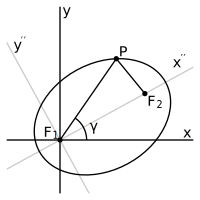
\includegraphics{5_e_orbit}} \hspace{0.2in} \resizebox{!}{2.0in}{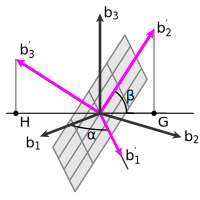
\includegraphics{5_e_orbit_plane}}
%\resizebox{!}{2.5in}{\includegraphics[trim=0.1cm 0.2cm 0.1cm 0.2cm, clip]{plane_2.png}} \hspace{0.2in} \resizebox{!}{2.5in}{\includegraphics[trim=2.0cm 0.3cm 2.0cm 0.3cm, clip]{plane_1.png}}
\end{center}
\caption{Left: The planet's orbit in the $x''y''$ system. Right: The planes of the planet and earth orbits.}
\label{F:orbits}
\end{figure}
%crop graphics in animate trim=<left> <bottom> <right> <top>, clip with includegraphics
Finally, let $\gamma$ be the angle between the positive $x'$ axis and the positive $x''$ axis as shown at left in Figure \ref{F:orbits}. Our first step is to find the change of basis matrix from $\CB''$ to $\CB'$. 

\begin{pactivity} \label{act:orbits_COB_1} Explain why the change of basis matrix $\underset{\CB' \leftarrow \CB''}{P}$ is given by 
\[\underset{\CB' \leftarrow \CB''}{P} = \left[ \begin{array}{ccc} \cos(\gamma)&-\sin(\gamma)&0 \\ \sin(\gamma)&\cos(\gamma)&0 \\ 0&0&1 \end{array} \right].\]


\end{pactivity}

More complicated is the change of basis matrix from $\CB'$ to $\CB$. 

\begin{pactivity} \label{act:orbits_COB_2} Now we look for $\underset{\CB \leftarrow \CB'}{P} = [[\vb'_1]_{\CB} \ [\vb'_2]_{\CB} \ [\vb'_3]_{\CB}]$. Assume that the plane $p$ in which the planet's orbit lies has equation $z = ax+by$. 
\ba
\item Explain why $\vb'_1 =  \cos(\alpha) \vb_1 + \sin(\alpha) \vb_2$. 

\item  The $x'$ axis is the intersection of the plane $z=ax+by$ with the plane $z=0$, so the equation of $x'$ axis in terms of $x$ and $y$ is $ax+by=0$. Now we determine the coordinates of $\vb'_2$ in terms of the basis $\CB$. 
	\begin{enumerate}[i.]
	\item Explain why the vector $[b \ -a \ 0]^{\tr}$ lies on the $x'$ axis. We take this vector to point in the positive $x'$ direction. This gives us another representation of $\vb'_1$ -- namely that $\vb'_1 = \frac{1}{\sqrt{a^2+b^2}} [b \ -a \ 0]^{\tr}$. 

	\item Explain why a vector in the plane $z = ax+by$ orthogonal to $\vb'_1$ is $\left[a \ b \ a^2+b^2 \right]^{\tr}$.

	\item  From the previous part we have 
\[\vb'_2 = \frac{1}{\sqrt{a^2+b^2+(a^2+b^2)^2}} \left[b \ a \ a^2+b^2 \right]^{\tr}.\]
Let $G = \left(\frac{b}{\sqrt{a^2+b^2+(a^2+b^2)^2}}, \frac{a}{\sqrt{a^2+b^2+(a^2+b^2)^2}}, 0\right)$ be the terminal point of the projection of $\vb'_2$ onto the $xy$ plane. Show that $\overrightarrow{OG}$ is orthogonal to $\vb'_1$. 

	\item Let $\beta$ be the angle between the plane $p$ and the $xy$ plane as illustrated at right in Figure \ref{F:orbits}. Explain why $||\overrightarrow{OG}|| = \cos(\beta)$. Then explain why 
\[\vb'_2 = [ -\cos(\beta)\sin(\alpha) \ \cos(\beta)\cos(\alpha) \ \sin(\beta)]^{\tr}.\]
(Hint: Use the trigonometric identities $\cos\left(A+\frac{\pi}{2}\right) =  -\sin(A)$ and $\sin\left(A + \frac{\pi}{2}\right) =\cos(A)$.)

	\end{enumerate}

	\item Finally, we find $[\vb'_3]_{\CB}$. The cross product of $\vb'_1$ and $\vb'_2$ is a vector orthogonal to $\vb'_1$ and $\vb'_2$, so 
\[\vb'_3 = \frac{1}{\sqrt{\left(a^2+b^2\right)^2+4a^2b^2}} \left[-a(a^2+b^2) \ -b(a^2+b^2) \ 2ab \right]^{\tr}.\]
Let $H$ be the terminal point of the projection of $\vb'_3$ onto the $xy$ plane as illustrated at right in Figure \ref{F:orbits}. 
	\begin{enumerate}[i.]
	\item Explain why the angle between $\vb'_1$ and $\overrightarrow{OH}$ is $\frac{\pi}{2}$. 
	

	\item Explain why $||\overrightarrow{OH}|| = \sin(\beta)$. (Hint: Use the trigonometric identity $\cos\left(\frac{\pi}{2}-A \right) = \sin(A)$.)
	
	\item Since the angle from $\vb_1$ to $\overrightarrow{OH}$ is negative, this angle is $\alpha-\frac{\pi}{2}$. Use this angle and the previous information to find the coordinates of the point $H$ and, consequently, explain why 
\[\vb'_3  = [ \sin(\beta)\sin(\alpha) \ -\sin(\beta)\cos(\alpha) \ \cos(\beta)]^{\tr}.\]
(Hint: Use the trigonometric identities $\cos\left(A - \frac{\pi}{2} \right) = \sin(A)$ and $\sin\left(A - \frac{\pi}{2}\right) = -\cos(A)$.)

	\end{enumerate}
	
\item Explain why the change of basis matrix $\underset{\CB \leftarrow \CB'}{P}$ from $\CB'$ to $\CB$ is 
\[\underset{\CB \leftarrow \CB'}{P} = \left[ \begin{array}{ccc} 
\cos(\alpha)&-\cos(\beta)\sin(\alpha)&\sin(\beta)\sin(\alpha) \\ 
\sin(\alpha)&\cos(\beta)\cos(\alpha)&-\sin(\beta)\cos(\alpha) \\ 
0&\sin(\beta)&\cos(\beta) \end{array} \right].\]

	\ea
	
\end{pactivity}

\begin{figure}[h]
\begin{center}
\resizebox{!}{2.0in}{
\includegraphics{5_e_ellipse_polar}} 
%\resizebox{!}{2.0in}{\includegraphics[trim=0.4cm 0.9cm 0.5cm 0.8cm, clip]{ellipse_polar.png}} 
\end{center}
\caption{Points on the ellipse in terms of angles.}
\label{F:ellipse_polar}
\end{figure}
With the change of basis matrices we can convert from any one coordinate system to the other. Note that all of the change of basis matrices are written in terms of angles, so it will be convenient to have a way to express points on our ellipses using angles as well. Given any point on an ellipse (or any point in the plane), we can represent the coordinates of that point in terms of the angle $\theta$ the vector through the origin and the point makes with the positive $x$-axis and the distance $r$ from the origin to the point as shown in Figure \ref{F:ellipse_polar}. In this representation we have $x = r\cos(\theta)$ and $y = r \sin(\theta)$. 

So we can start in the $x''y''$ coordinate system with the coordinate vector of a point $\left[\overrightarrow{OP}\right]_{\CB''} = [ r\cos(\theta) \ r\sin(\theta) \ 0]^{\tr}$. Then to view this point in the $xy$ system, we apply the change of basis matrices 
\[\left[\overrightarrow{OP}\right]_{\CB} = \underset{\CB \leftarrow \CB'}{P} \underset{\CB' \leftarrow \CB''}{P} [ r\cos(\theta) \ r\sin(\theta) \ 0]^{\tr}.\]
Of course we can also covert from $\CB$ coordinates to $\CB''$ coordinates by applying the inverses of our change of basis matrices. 



